\chapter{xHCI Stack Implementation}

The structure of the xHCI driver is quite straightforward, as it tries to fit
into the scheme of how hardware and the rest of HelenOS works. We decided to
use the existing library \lib{libusbhost} to reduce code duplication with
other HC drivers. It came out that this library needs a lot of changes to
support us in this goal, but that's for chapter \ref{usb-refactoring}.

The USB host controller driver using \lib{libusbhost}, xHCI included, serves as
a connecting layer between the hardware and library, and exposes its bus
interface.

\begin{figure}[h]
	\centering
	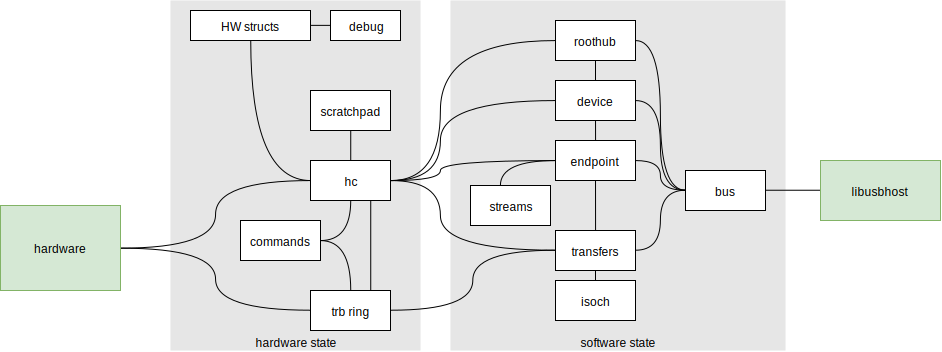
\includegraphics[width=0.8\textwidth]{xhci-architecture}
	\caption{The modules of xHCI driver}
\end{figure}

The scheme is not at all strict, we're in a C world, there are dependencies
almost everywhere -- take it as an informal overview to get an idea.

The whole driver can be split into two parts. The left one takes care about the
hardware perception of what's going on, the right one is about managing the
software structures and memory.

We start with describing the modules in the hardware part, as their
functionality is clear. Their order follows the order in which they were
implemented.

\section{Hardware Structures}

The \file{uspace/drv/bus/usb/xhci/hw\_struct}{hw\_struct} directory contains C structures
that represent registers and control structures used by the xHC. The memory layout of the
structures is defined by the xHCI specification and thus the files in this directory should
be mostly treated as read-only.

\subsection{Registers}

The register structures (defined in \file{uspace/drv/bus/usb/xhci/hw\_struct/regs.h}{regs.h})
represent hardware registers presented by the xHC to system software
implemented as Memory-Mapped I/O space. They can be divided into four categories as follows:
~
\begin{description}
	\item[Capability registers]
		These specify read-only limits, restrictions and capabilities of the specific
		xHC implementation used.
	\item[Runtime and Operational registers]
		These specify the current xHC configuration and runtime modifiable state.
	\item[Extended capabilities]
		These specify optional features of the current xHC implementation.
	\item[Doorbell array]
		An array of up to 256 doorbell registers, which supports up to 255 USB devices
		or hubs. Each doorbell register provides the software with a mechanism for
		notifying the xHC if it has slot or endpoint related work to perform.
\end{description}

In our implementation, all of these can be accessed through the \struct{xhci_hc_t} structure and
can be modified through it using the register handling macros defined in
\file{uspace/drv/bus/usb/xhci/hw\_struct/regs.h}{regs.h}. Note that not all register bits can be
manipulated freely by the system, some impose restrictions:
~
\begin{description}
	\item[RO, Read-only]
		Register bits are read-only and cannot be altered by system software. An example
		is the \textit{CAPLENGTH} register (see \xhci{5.3.1}).
	\item[RW, Read-Write]
		Register bits are read-write and can be altered by system software. An example
		is the \textit{USBCMD} register (see \xhci{5.4.1}), in which some bits or bit ranges
		are RW (and some are read-only).
	\item[RW1C, Write-1-to-clear]
		Register bits indicate status when read, a set bit can be cleared by writing
		a '1', writing a '0' to such register bit has no effect. An example is
		the \textit{Event Interrupt} bit in the \textit{USBSTS} register (see \xhci{5.4.2}) which is set
		to '1' by the xHC when an interrupt occurs and can be cleared by the driver
		by writing '1' to it once the event is scheduled for handling.
	\item[RW1S, Write-1-to-set]
		Register bits indicate status when read, a clear bit can be set by writing
		a '1', writing a '0' to such register bit has no effect. Examples are the
		\textit{Command Stop} and \textit{Command Abort} bits of the \textit{CRCR} register
		(see \xhci{5.4.5}).
\end{description}

This is not an exhaustive list of access attributes, for the entire list, see \xhci{5.1.1}.

\subsubsection{Register access macros}

Registers are accessed very often in all hardware-related modules. We felt that
there is a need to centralize the information defined in specification,
especially the subdivision of registers to individual fields. There are several
common solutions to this problem.

Probably the most common one, which we also considered at first, is defining
two constants for every such field: mask and shift. When one needs to read
a field, they read the value of the register, use the mask to select bits, and
then shift the value according to the shift macro. To write a field, one reads
the value of the whole register, uses the bitwise negation of the mask to copy
surrounding bits, then shift the value to be written into its place. This
solution is simple to understand, yet hard to use correctly. There's a lot of
repetition, the more if you consider endianity (HelenOS is targeted also on Big
Endian platforms, while the USB world is Little Endian).

Another possibility is to define macros for reading and writing every single
field. That idea was discarded in its very beginning. We wanted a solution,
that requires only one definition per field, cannot be used in a wrong way and
is sensibly short to write. So we came up with the register access macros. The
best introduction is probably by an artificial example:

\begin{listing}[h]
\begin{code}
#define XHCI_SOME_FIELD            usbreg, 32, RANGE, 13, 7

unsigned field = XHCI_REG_RD(hc->op_regs, XHCI_SOME_FIELD);
XHCI_REG_WR(hc->op_regs, XHCI_SOME_FIELD, 42);
\end{code}
	\caption[An example of using register macros]{On the first line, we read
	bits 13 to 7 of the field \mintinline{c}{hc->op_regs->usbreg} to
	a variable, and then change the same bits in the register to a value 42.}
\end{listing}

All the definitions of macros like \macro{XHCI_SOME_FIELD} relevant for xHCI
are contained in the header file \header|hw_struct/regs.h|. The definition
contains all the information necessary to access the field. It says that the
register field is contained in a field \struct{usbreg} of an operational
register structure (the one \mintinline{c}{hc->op_regs} points to), the
structure field is a 32 bit wide dword, and that the register field is
contained in bits 13 to 7 of it.

The primary principle used to implement these preprocessor macros is the
specific order of macro expansion in C. In the example, the register definition
macro is used as an argument to the \macro{XHCI_REG_RD} macro. Both macros are
expanded in a breadth-first fashion, producing just another preprocessor macro
\macro{XHCI_REG_RD_INNER(hc->op_regs, usbreg, 32, RANGE, 13, 7)}. You can see
that one argument is expanded to several arguments for the inner macro. What
happens next is pretty simple. The \macro{RANGE} argument token is glued to
a prefix, producing a name for another macro, which selects between
implementations for whole fields, bit ranges and individual bit flags. The
\macro{XHCI_REG_RD_RANGE} then extracts the specified bits read from whole
field. The size argument is needed to properly handle endianity. All other
top-level macros (\macro{XHCI_REG_WR}, \macro{XHCI_REG_SET},
\macro{XHCI_REG_CLR}, \macro{XHCI_REG_MASK} and \macro{XHCI_REG_SHIFT}) operate
on the same principle.

We think we have achieved our goal. These macros are a bit hard to understand but
very easy to use, and require just one line of definition per field. Looking
back though, the work was probably not worth it -- the registers are not used
that much to justify existence of register definition of every single register
field. But it is already done and shall there be a need to access more registers,
it's easily accessible without thinking how to select the proper bits and
ensure the correct endianness. And even if there wasn't, it serves as a nice
showcase of what are preprocessor macros capable of.

\subsection{Contexts}

Contexts (defined in \file{uspace/drv/bus/usb/xhci/hw\_struct/context.h}{context.h})
are control structures that represent devices and their configuration as well
as the parameters of the communication between the xHC and system software. The
\struct{xhci_hc_t} structure contains the \textit{Device Context Base Address Array} (DCBAA), which
holds up to 255 pointers to device contexts at indices 1 through 255 and a pointer to
the scratchpad array (see \ref{sec:scratchpads}). Each device context contains a slot
context (used to describe the device as a whole, represented by \struct{xhci_slot_ctx_t}) and
31 context for each endpoint (represented by \struct{xhci_ep_ctx_t}). Most of these contexts
will be described in more detail in the following sections.

% TODO device & input ctx problem with 32-bit and 64-bit?

\section{Debug}

Since both the internal state of the xHC and its capabilities are often described by
a handful of bits located in a packed 32-bit register, we needed a way to monitor these
values in a human readable form. The \file{uspace/drv/bus/usb/xhci/debug.h}{debug.h} and
\file{uspace/drv/bus/usb/xhci/debug.c}{debug.c} files contain a set of register dumping
functions that use the register reading macros described in the previous section to print
the values of all the bit sets contained in a register to the driver's log. They also contain
auxiliary functions that are used to convert numeric codes to their meaning in a string form and
functions that dump the contents of a hardware structure (such as \struct{xhci_endpoint_ctx}).

These functions have proved to be of great use and should any future maintainer of the
HelenOS xHC stack find themselves in a bug ridden situation, putting these functions to
the areas of code they suspect of mischievous deeds might be a good starting point.

\section{TRB Ring}

One of the primary means of communication with the HC, apart from register
interface, are the TRB rings. Their management is fully contained in the TRB
ring module. Before we dive into the implementation details, let us first
describe how these rings works.

\subsection{Architectural overview}

\emph{Transaction Request Block}, everywhere else abbreviated as TRB, is
a fixed-size structure with contents of variable type. The most notable
exception being a \emph{TRB Type} field. Each of the 64 TRB types defines the
other fields that are contained inside a TRB. Most commonly, it just contains
a pointer to another buffer together with the size of the buffer, or a result
of an operation.

\emph{TRB Ring} is then a circular queue comprised of individual TRBs. The main
difference from older HCIs is that TRBs are required to be contiguous in
memory, forming a \emph{TRB Ring Segment}. It is of course needed to link the
two ends of the segment together, one must use a special TRB type called
\emph{Link TRB}, which serves as a glue between the end and the beginning of
a segment. It is not required from the ring to be composed of only one segment,
but then special precautions must be taken.

TRB Ring is used in many instances during the lifetime of the Host Controller.
There are two special instances though: the \emph{Command Ring} and the
\emph{Event Ring}. The command ring serves as a channel to command the HC, and
the command interface is described in more depth in section \ref{sec:commands}.
The event ring is asynchronously read to retrieve results of commands,
completed transactions and so on, as the primary information channel from HC to
host. Actually, there can be more than one instance of Event Ring, but that
requires the host to be able to recognise multiple interrupts, which is not
supported in the current version of HelenOS. The event subsystem is further
discussed in the section \ref{sec:events}. The third type of a~ring,
a~\emph{Transfer Ring}, is used for every pipe endpoint on the bus - either
Endpoint or a Stream. These are used by the Transfer module, described in
section \ref{sec:transfers}. For now, let's discover the mechanics of the rings
themselves, regardless of their type.

As already said, TRB ring is a circular queue. It always has one producer and
one consumer of TRBs. Every ring implicitly defines two pointers: the enqueue
pointer and the dequeue pointer. The producer uses the enqueue pointer to
enqueue TRBs and the consumer uses the dequeue pointer to dequeue them. The
pointers are not shared between the host and the Host Controller. Instead,
every TRB has one bit with special semantics, the \emph{Cycle Bit}. The
transition between values of TRB Cycle Bit of individual TRBs defines the
value of Enqueue pointer. An example situation is shown on the figure
\ref{fig:ring-simple}.

\begin{figure}[h]
	\centering
	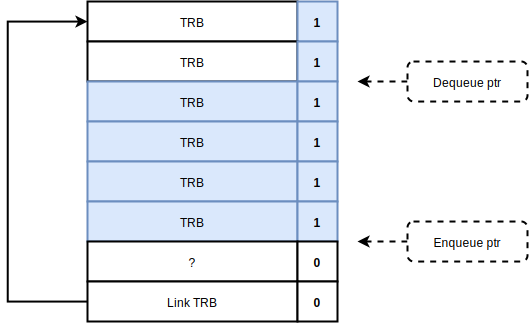
\includegraphics[width=0.6\textwidth]{ring-simple}
	\caption{A simple example of a TRB ring.}
	\label{fig:ring-simple}
\end{figure}

It is important to understand that the consumer cannot write to the ring and
thus cannot change the value of the Cycle Bit after it processes a TRB.
Therefore, the position of the dequeue pointer must be signalized by other
means. Furthermore, there has to be a mechanism to stop the consumer from
considering the TRBs in the beginning of the segment as enqueued, after it
wraps around the segment boundary. The enqueue pointer is not defined by
a transition from one to zero, but more generally by a transition from
\emph{Producer Cycle State}, \texttt{PCS}, to \texttt{\textasciitilde PCS}.
This bit is kept in the memory of the producer. Similarly, there exists
a \emph{Consumer Cycle State}, which has the same value as \texttt{PCS} had in
the moment when the value of the enqueue pointer was the same as the current
value of the dequeue pointer.

The Link TRB contains a \emph{Toggle Cycle} flag, which if set, instructs both
producer and consumer to toggle its cycle state when this TRB is
enqueued/dequeued (Link TRBs are not necessarily fixed in place, they are queue
members as any other TRB). There shall always be an odd number of Link TRBs
with the Toggle Cycle flag set on the ring.

We haven't yet covered how the producer can be aware of the dequeue pointer
value. In case of Command and Transfer rings, the producer is the Host
Controller. Every finished command or transfer is denoted by an Event TRB
placed on the Event Ring. This Event TRB usually contains the physical address
of the TRB on the respective Command or Transfer ring. This way the producer
knows that the dequeue pointer value is not less than the reported value.
Similarly, when the host processes an Event TRB on the Event Ring, it shall
report the physical address of the TRB processed by writing the value into
a dedicated register.

Also, the Event ring differs a bit in the usage of multiple segments. As the
Host Controller is obviously unable to allocate ring segments and map them into
virtual address space of the driver, and it's even not possible to allow the
host to write Link TRBs onto the ring, which is otherwise read-only for the
host, a~different approach has to be used. Instead of the segments being linked
together, the host preallocates a number of segments, and an \emph{Event Ring
Segment Table}, which is another structure defined by the specification. The
segments' addresses and sizes are written into the table, and the address of
the table is written to a dedicated register. At the time of the write, the
ownership of all the buffers is transferred to the Host Controller.

\subsection{Implementation}

As the requirements imposed by the specifications are quite strict, there's not
much freedom in the implementation. However, there were some decisions to be
discussed.

First, we decided not to restrict ourselves on single-segment rings as
other existing implementations do, though we haven't implemented runtime
scaling yet. Second, we implement and use three types of TRB rings;
the third one being a simplified TRB ring used by the host from both sides. Its
purpose is better described in the section \ref{sec:events}. The three
implementations are somehow separate, but because they share principles, they
reside in a common module.

The containing structures are called \struct{xhci_trb_ring_t},
\struct{xhci_event_ring_t} and \struct{xhci_sw_ring_t} for Command/Transfer
rings, Event ring and host-only rings, respectively. Despite their name, these
structures only represent the ring in host memory, and are not the structures
given to the hardware. Let's walk through them one by one.

\subsubsection{Command and Transfer Rings}

These rings are prepared to be multi-segment. They contain a list of
\struct{trb_segment_t} structures, which represent one ring segment. The
segment itself is allocated as a DMA buffer (sect. \ref{sec:dma-buffers}) of
size \macro{PAGE_SIZE}. The space for TRBs is in the beginning to ensure
alignment. At the end, there is a small footer keeping the physical address of
the segment and a link to the segment list. There are helper functions to
manage segments.

To avoid keeping the \struct{dma_buffer_t} structure inside the segment and
wasting precious DMA-accessible memory, the structure is reconstructed in order
to be freed in \fnc{trb_segment_free}. We agree that this violates the
encapsulation of DMA buffers, but consider this the lesser evil.

The main runtime interface to rings of this kind is the method
\fnc{xhci_trb_ring_enqueue_multiple}, used to enqueue a contiguous array of
TRBs (referred to as Transfer Descriptor, TD) onto the ring. As this method
must not block to be usable in atomic contexts, it first performs a dry run to
check if there is enough space on the ring, then rollbacks and actually
emplaces the TRBs. Because it might be needed to interleave the Transfer
Descriptor with multiple Link TRBs, it is not possible to simply calculate the
free space in advance.

Because the caller of this function needs to know the physical address of the
TRB enqueued to pair it with the completion event, the address is assigned to
an output argument. If there are multiple TRBs to be enqueued, the one with
\emph{Interrupt On Completion} flag is reported -- because that's the one that
will generate the event.

The second crucial part of the interface is the function
\fnc{xhci_trb_ring_update_dequeue}, by which the dequeue pointer advancement is
announced to the ring. As the rings need to be configured to the hardware
somehow, there is also a function called
\fnc{xhci_trb_ring_reset_dequeue_state}, which is used to reset the ring and
also return a value used to configure the ring in the HC -- a physical pointer
mixed with the initial Consumer Cycle State.

\subsubsection{Event Ring}

The implementation of the event ring is fairly simple, with the main
interaction point being the function \fnc{xhci_event_ring_dequeue}. This
method, symmetrically to the TRB ring enqueue, does not block if the ring is
empty, but returns \macro{ENOENT} instead. This structure also contains the
Event Ring Segment Table.

\subsubsection{Software Ring}

This structure is to be used as a buffer for exchanging information between
different fibrils of the driver. It is an ordinary implementation of a circular
blocking queue made for TRBs. It uses the Cycle bit inside TRBs to indicate
active entries, because both sides are allowed write to the ring when the guard
is locked. Also, this ring is not allocated using DMA buffers, because it is
not expected to be accessed by hardware.


\section{Scratchpad}
\label{sec:scratchpads}

Scratchpads are buffers that an xHC implementation can request from the system software
for its internal needs. The size of these buffers is specified in the \textit{PAGESIZE} register
found in the operational register set defined in \struct{xhci_op_regs}.

The amount of buffers requested by the xHC is specified in the \textit{Max Scratchpad Bufs Hi} and
\textit{Max Scratchpad Bufs Lo} registers of the second set of structural parameters (\textit{HCSPARAMS2},
see \xhci{5.3.4}) defined in \struct{xhci_cap_regs}.

The allocation of these buffers takes place as part of the host controller initialization,
specifically in \fnc{hc_init_memory}, which calls \fnc{xhci_scratchpad_alloc}. The pointers
to these buffers are then passed to the xHC in the \textit{Scratchpad Buffer Array}, pointer to which
occupies the first index of the \textit{Device Context Base Address Array} (dcbaa field of
\struct{xhci_hc_t}).

Our implementation originally implemented these as a standalone structure \struct{xhci_scratchpad_t},
which served mainly for the purposes of resource management by keeping both the physical addresses
for the xHC and the virtual addresses for deallocation. This was, however, later refactored to use
\struct{dma_buffer_t}, which is part of \lib{libusbhost} and was created for the same purpose.

Once the xHCI driver finishes its execution, the scratchpad buffers are deallocated by a call to
\fnc{xhci_scratchpad_free} as part of \fnc{hc_fini}.


\section{Commands}
\label{sec:commands}

The xHC offers an independent command interface. During operation, the xHC
driver uses this interface to manipulate device slots, devices and endpoints by
executing various commands provided by a unified command subsystem. This
section provides details on the structure and implementation of this subsystem.


\subsection{Execution Workflow}

The xHC command interface consists of a TRB command ring and a command doorbell
register. Commands are executed by placing various command TRBs onto this ring,
forming a \textit{Command Descriptor}.

After placing the respective TRBs and writing to the xHC command doorbell
register, the descriptors on the command ring are sequentially processed by the
xHC, resulting in either failure or successful completion. The result of every
command descriptor is reported back to the xHCI driver in the form of a
\textit{Command Completion Event} placed onto the primary event TRB ring.

After writing into the xHC command doorbell register and before receiving the
respective command completion event, the xHCI driver can attempt to abort the
issued command. Such action might be of use for instance if the command
completion event does not arrive within a set time period.

Note that this section intentionally omits hardware technical details, which are
not instrumental in understanding the command subsystem. For further hardware
documentation of the xHC command interface, refer to \xhci{4.6}.


\subsection{Structure}

The xHCI driver command subsystem instance is represented by the
\struct{xhci_cmd_ring_t} structure which exists throughout the entire duration
of the xHCI driver's lifecycle. The purpose of this structure is to maintain and
manage the command TRB ring and to keep track of enqueued command descriptors.

Individual command descriptors are represented by the \struct{xhci_cmd_t}
structure. In this structure are stored high-level parameters of the command as well as
the command TRB, which is placed onto the command ring when the command is
executed. While the high-level command parameters are kept directly in this
structure, the hardware-related internals are kept in a substructure, which is
commonly referred to as \textit{command header}. The purpose of this separation
is to stress that the header contents are to be exclusively accessible to the
command subsystem, while the rest of the structure remains accessible to
the entire xHCI driver.

Besides data structures, the command subsystem offers a centralized command
completion event handler function -- \fnc{xhci_handle_command_completion} --
which is called by the event subsystem in case a \textit{Command Completion
Event} is encountered.

The last major component of the command subsystem are functions used to generate
and schedule commands on the xHC. These functions produce valid instances of the
\struct{xhci_cmd_t} and place their respective TRBs onto the command ring
managed by the \struct{xhci_cmd_ring_t} structure, requesting either blocking or
non-blocking semantics for waiting on their completion. These functions are
described in detail in the next section.


\subsection{Command Lifecycle}

\subsubsection{Issuing Commands}

By design, the internal logic of the command subsystem is kept opaque with
respect to other components of the driver. A notable example of this is the
mechanism for command scheduling.

Commands are usually issued by the HC component of the xHCI driver. At the time
of issuing, the information required can be broken down into three groups:
%
\begin{description}
	\item[Command Type]
		One of the 15 commands supported by the xHC command interface.
	\item[Command-specific Parameters]
		The number, type and semantics of these parameters depend on the
		specified command type.
	\item[Completion Semantics]
		This is the desired behavior of command execution.

		In the \textit{blocking mode}, the call to issue the command will block
		the calling fibril until the completion event is received.

		On the other hand, in the \textit{non-blocking mode}, the fibril will
		only be blocked until the command is issued -- the command subsystem
		will take the ownership of the command and deallocate it when the
		completion event arrives. This mode is meant for commands which do not
		require completion event handling and involves more complicated memory
		management since the command subsystem is responsible for freeing the
		command after the completion occurs.
\end{description}

Depending on the desired completion semantics of the issued command, the HC
component calls either the \fnc{xhci_cmd_sync} or \fnc{xhci_cmd_async}
function and passes it a configured instance of the \struct{xhci_cmd_t} structure.
Upon such call, the command subsystem will execute an internal command handler
function, which copies the high-level command-specific parameters configured by
the issuer, and use their values to construct a command descriptor consisting of
TRBs.

At this point, the \struct{xhci_cmd_ring_t} structure is modified and the new
command descriptor is placed onto the TRB ring. The corresponding instance of
\struct{xhci_cmd_t} is added to the active command list and depending on the
completion semantics, the issuing fibril is either suspended or continues
execution regardless of the completion event.


\subsubsection{Handling Completion}

When a command is completed, a \textit{Command Completion Event} is generated by
the xHC. This event is detected by the event subsystem, which in such case
triggers the \fnc{xhci_handle_command_completion} function.

This function extracts the address of the completed command descriptor and uses
it to find a matching instance of the \struct{xhci_cmd_t} structure in the
active command list.

Depending on the desired completion semantics, the command subsystem either
wakes the sleeping issuer fibril, or discards the non-blocking command from the
memory.


\subsubsection{Aborting Commands}

The command subsystem defined by xHCI contains a mechanism to trigger early
command abortion. It is not guaranteed to be effective for all commands, just
for commands control of which is out of HC's hands. A good example might be the
\macro{SET_ADDRESS} command, which issues the USB control request
\emph{SetAddress}, and waits for the device's response. Such command blocks
until the response is received. If the software, for any reason, wants the
command to be aborted, it can write 1 to the \macro{CA} bit of the
\emph{Command Ring Control Register}.

When the HC is triggered by a command abortion, it places a \emph{Command Ring
Stopped} event on the primary event ring and halts command processing. The ring
can be started again by ringing its doorbell. If a command was actually
aborted, a corresponding \emph{Command Completion Event} with status
\emph{Command Aborted} is placed first.

We decided to set a fixed timeout for every command, regardless of its
possibility to block, arbitrarily chosen as 10 seconds. That gives a generous
amount of time for the HC to finish a command. When this timeout is over,
a command is aborted.

Here comes the catch: the driver is not able to choose which command is to be
aborted -- it is always the one currently processed. Usually, it's the one that
blocks the pipe, but it means that the driver cannot simply place a timed
constraint on a command execution. To reflect the hardware semantics, all
fibrils that expire the timeout behave the same: they trigger a command
abortion, wait for the command ring to be stopped, then start it again.

To orchestrate several fibrils trying to schedule new commands, waiting for
commands to be completed and also the one handling an interrupt, a simple state
machine with synchronization is incorporated. In case the command ring is
being restarted, newly issued commands are delayed to prevent the doorbell from
being rung unexpectedly. When there are multiple fibrils with an expired timeout
while the abort is already triggered but not yet finished, they retract and
wait for the full timeout period again.

That common execution path is enclosed within a function called
\fnc{try_abort_current_command} (static for the command subsystem). As it's hard
to force a command to stall, we haven't had many opportunities to test the
behavior. Usually, the mechanism was triggered by a deadlock in our code, which
didn't magically disappear when a command was aborted. Also, the commands
always finish on time in a virtual environment. At the time of writing this
documentation, there has been only one observed legitimate occurrence of
a command stall on real hardware. The abort mechanism did its job well that day.

\subsection{Usage Examples}

Since the command subsystem is used at a multitude of places in the HC
component, it has been the goal of the authors to make its usage elegant and
effortless. For that reason, a dedicated inline notation syntax powered by
preprocessor macros has been devised and implemented. This is demonstrated in
Listing \ref{lst:command-usage}.

\begin{listing}[h]
	\begin{code}
		xhci_hc_t * const hc;

		/* Issue a "Set TR Dequeue Pointer" command synchronously. */
		const int result = xhci_cmd_sync_inline(hc, SET_TR_DEQUEUE_POINTER,
		    /* Command-specific arguments use struct initializer. */
		    .slot_id = slot_id,
		    .endpoint_id = dci,
		    .stream_id = stream_id,
		    .dequeue_ptr = addr,
		);

		/* At this point, the command is completed with `result`. */
	\end{code}
	\caption[Usage example of xHCI driver inline command syntax.]{Usage example
	of the xHCI driver command subsystem inline  syntax. This snippet issues a
	\textit{Set TR Dequeue Pointer} command to the HC in blocking mode. Note
	that the command initialization, configuration and finalization is handled
	by the inline macro syntax.}
	\label{lst:command-usage}
\end{listing}



\section{Host Controller Module}

This module contains the mixture of things that didn't fit anywhere else, or
didn't deserve their own submodule. We tried to move the ``xHCI specification
quirks'' here, so that other modules rely only on the semantics and overview of
the xHCI, and don't care that much about the exact technical details. Of
course, it's not strictly possible, because the whole driver is about technical
details of xHCI.

\subsection{Initialization}

A substantial part of this module handles the initialization of the controller.
When the xHC device is added, several steps needs to be done. Lets walk through
them in order. The DDF callback \fnc{dev_add} is handled by the
\lib{libusbhost} library, so the story begins there.

\begin{enumerate}
\item
	At the very beginning, the supplementary structures are allocated in the
	DDF device node. These structures accompany the entire lifetime of a driven
	HC.

\item
	The DDF control function is created. Through it, the user may command the
	HC driver.

\item
	The hardware resources such as MMIO space or IRQ number are obtained from
	the parent device (usually PCI driver).

	Now, the structure and hw resources are handed out to the xHCI driver for
	the first time, to do its initialization.

\item
	The MMIO range needs to be mapped, and the proper register areas found.
	xHCI specifies several areas of MMIO registers, with variable offsets
	between them. We cache the pointers to the areas inside the
	\struct{xhci_hc_t} structure to make the access convenient.

\item
	The roothub structures are initialized. The number of ports is obtained and
	memory for state machines is allocated.

\item
	Extended capabilities need to be parsed soon enough, as they contain some
	crucial information. Namely the information about legacy support, but also
	the protocol versions supported on individual roothub ports.

\item
	A lot of memory structures are to be initialized now. The \emph{DCBA}
	array, event ring, scratchpads, command ring, the device-keeping array and
	also the event worker fibril.

	After all of that, the basic driver initialization is completed, and the
	execution returns to the library.

\item
	The interrupts need to be enabled, if they are available. The driver is
	given an opportunity to generate the bottom-half IRQ handling code, and
	than the code is registered in the kernel. Shall any of these steps fail,
	the failure is not critical, the interrupts are just marked unavailable.

\item
	If the HC is being controlled by the BIOS (denoted by the extended
	capability), it needs to be claimed.

\item
	The HC is started. In case of xHCI, an initialization sequence as described
	in the specification is performed. The HC is reset to transition into
	a known state. The addresses of the memory structures are configured. If
	the interrupts are available, the interrupter 0 is enabled. Finally, the HC
	is started by setting a bit in the operational registers.

\item
	Before the control is returned to the library, all roothub ports are
	checked for a change, because the reset changed their connection state,
	but the Port Change Events had no ring to be written on.

\item
	If the interrupts are not available, a replacement polling fibril is
	started.

\item
	The roothub is to be set up. Other HCs using virthub must undergo an
	enumeration process, so this must be done after the initialization is fully
	completed. In case of xHCI, this step is skipped.
\end{enumerate}

A symmetric reverse sequence is performed to make the HC stopped again. This
functionality is however not tested, because PCI devices are not hotpluggable,
not even in QEMU.

\subsection{Events}
\label{sec:events}

Another functionality provided by the HC module is the first line of handling
events. Events are the primary information channel from the device to the host.
Every synchronous operation needs to be finished by waiting for an event.

The tricky part in handling events is, again, the synchronization. Event
handlers must not issue operations, which would wait for another events. The
problem is that this event dependency is inevitable in some cases. Let us
describe two scenarios which will explain the complexity of the final solution.

First, there are the Port State Changed Events. Handling these events usually
involves device enumeration -- that is however handled in a separate fibril.
Its even not the reset completion which would create a deadlock -- if it is
expected, all the locks are unlocked. The main problem is a device
disconnection while the enumeration is still in progress -- when it happens,
the event handling fibril must wait until the enumeration fibril terminates.
But the enumeration might be in the later phase, in which it issues commands.
In order to terminate, a command must be completed. That introduces
a dependency, which cannot be simply removed. Because of it, Port Change
Detected Events and Command Completion Events must be handled independently on
each other.

Similarly, the enumeration process involves fetching descriptors from the
device. That introduces another dependency, this time between Transfer
Events and Port Change Detected Events. Neither these two can be handled
sequentially.

The last dependency is between Command Completion Events and Transfer Events,
forming a dependency triangle. This one might not be that obvious, but it is
there and cannot be avoided easily. The handler of the Transfer Event needs to
obtain a reference to an endpoint. To ensure coherency, the reference must be
created while the endpoint is still registered, in a critical section. The same
critical section that protects the endpoint unregistration -- which needs to
abort currently running transfers.

In order to avoid deadlock, all three types of events need to be processed
separately. We achieve it by processing only so-called fast events (Command
Completion, MFINDEX Wrap) in the interrupt handler, and route the Port Change
Events and Transfer Events to two Software TRB Rings (see section \ref{sec:sw-rings}),
from which two other worker fibrils dequeue and handle the events independently.

\subsection{Commands abstraction}

Although the command interface have a module on its own, there are situations
where the specific commands used are a technical detail hiding the actual
semantics of the operation. To give an example, to inform the HC about dropping
an endpoint, one must issue the \emph{Configure Endpoint} command with a flag
set. Also, some commands require an input context with a proper content, some don't.

The rest of the Host controller module tries to cover this implementation
details and offer a more intuitive interface. Although the device and endpoint
modules do fill the contexts on their own (being also a technical detail), the
decision whether its needed to fill an input context is left to the HC module.

\section{Root Hub}

The purpose of this module is very simple -- take care of the root hub. Before
we explain how our roothub works, let's have a look on why and how other HC
drivers handle it.

The main problem a hub driver faces is a synchronization one. When a new device
is detected, it needs to be enumerated. Enumeration process in the case of USB 2.0
devices requires the hub to reset the port the device is attached to, to move
it to the \state{Default} state, when it's listening on the default address 0.
When the port reset is triggered, the hub must wait until the port reset is
complete. During the whole process, the device can be disconnected, and the
port reset will never be completed. Furthermore, the completion of port reset
is indicated by the same means as port connection, resulting in a deadlock in
the na\"ive solution. The proper solution therefore involves spawning new
fibrils and nontrivial synchronization.

All four HC drivers (UHCI, OHCI, EHCI and VHC) are using a virtual roothub. In
principle that means that they create a virtual USB device, which is listening
at the default address in the beginning, and trigger an enumeration process.
Then there is a little branch in transfer scheduling, that takes transfers
directed to the same address as the virtual device's, and delivers them by
calling a function instead. The virtual device behaves exactly like a real USB
hub would -- it has its standard descriptors, reply to setup requests and so
on. So it enumerates like a USB hub would, and creates a DDF device, which is
taken by the \texttt{usbhub} driver. The driver then handles the virtual
roothub like any other hub, by sending USB control transfers. The virthub
module translates USB transfers to callbacks, which are implemented by
individual HC drivers to read and modify register space of the Host Controller.

This solution is very clean in design, regarding that root hub functionality is
exactly the same as any other hub's, but just controlled by MMIO mapped
registers instead of USB packets. It is even recommended by the USB 2.0			% TODO: Link to USB2 spec
specification to embody this solution. But that's pretty much the only advantage
this solution has. One has to write a lot of code to even implement the
callbacks, not mentioning the virthub module itself. And a lot of code always
comes with bugs. Also, while having no real performance impact, it requires
several context switches, IPC calls, bouncing memory buffers and a lot of
unnecessary allocations to clear one bit in the register space (USB hubs
operate by setting and clearing so-called Features, indicating e.g. that
a connection on port changed). But it needs to be stressed more that this
performance impact is mitigated by the fact that real hubs use real USB transactions
above that and that hub interaction is very sparse.

We searched for a solution that would keep the cleanness in terms of shared
functionality between usbhub driver and roothub and decided to move the port
state machine and related fibril synchronization into the USB library. That
cleanly separates the hardest part of handling hub port changes from the code
that is actually handling them and enumerating the devices. This state machine
is used by both the xHCI roothub and also by the rewritten usbhub. More
information about this new module can be found in section \ref{hub-port-refactoring}.

One more thing related to the xHCI roothub, which we crossed while debugging on
real hardware: the USB hub have a bit dedicated to indicate that a port is
enabled (PED), and the port can be disabled using it. Counterintuitively, the
port is disabled by writing a 1 to it. Even worse, this bit is in the same
field as the change bits with RW1C semantics are -- which means that the
standard approach of reading and writing back the value read fails hard. This
took us several hours to discover, because the port reset was completed
successfully, but right after that, the device was inaccessible, even when we
didn't do anything with it yet. To make matters more complicated, QEMU ignores
this bit completely, so the code worked fine in a virtual environment.

\section{Bus Module}

% TODO: After the device will be split, will there be anything interesting to write about?

\subsection{Device}

% TODO: Enumeration, device context

\subsection{Endpoint}

% TODO: Contexts, rings

\section{Transfers}
\label{sec:transfers}

The xHC uses transfers to abstract USB communication. Every call to
\fnc{usb_write} and \fnc{usb_read} is accomplished by creating a transfer,
setting it up, handing it to the xHC and waiting for transfer completion. This
section describes the code structure and implementation details of the xHCI transfer
subsystem.

\subsection{Executing Transfers}

The xHC is responsible for communicating with USB devices using USB packets.
These USB packets are created from the data given to the xHC through the
transfer rings by the software. The software isn't required to split the
transfer into USB packets, the xHC takes care of that.

Each transfer is formed by a \textit{Transfer Descriptor}, which is a sequence
of TRBs with a chain bit set. This allows the software to schedule a transfer
containing larger data, or data not stored in continuous memory. Each TRB
points to a single continuous buffer of data (in physical memory) and specifies
the buffer's size. This buffer must be accessible to the hardware and it's
physical address needs to be set to the TRB.

Every endpoint uses a single transfer ring (with the exception of streams)
initialized during the endpoint configuration. This transfer ring is passed to
the xHC by the endpoint context. The software is not allowed to modify the
transfer ring except when it wants to enqueue more transfer descriptors. If the
software requires to modify the ring, it has to first stop the endpoint using
the command interface, and after the modification is done, it has to use the
evaluate context command to communicate the changes to the xHC.

After the software puts a transfer descriptor on the transfer ring, it rings
the doorbell associated with the device and the endpoint. This notifies the xHC
and causes it to schedule the endpoint and process the transfer.

After the transfer descriptor finishes processing, the xHC can optionally
notify the software of the completion by generating a \textit{Transfer Event}
on the event ring with the completion code set to reflect the result. By
default, this only happens if the TRB processing ends with an error.
The software can set the \textit{IOC (Interrupt on Completion)} bit if it needs
to be notified regardless of an error happening.

\subsection{Lifecycle}

Every transfer is represented by a single instance of \struct{xhci_transfer_t}
structure. This structure encapsulates the \struct{usb_transfer_batch_t}
structure, which is used by \lib{libusbhost} to schedule USB batches. Its
lifetime is managed by the library calling the bus operations.

After the library allocates and fills up the \struct{usb_transfer_batch_t}, it
schedules the transfer. This is where the xHCI takes control over the transfer.
The transfer is processed in \fnc{xhci_transfer_schedule}, where it is split
into TRBs, the correct bits are set depending on the transfer type, TRBs are
enqueued and the doorbell is rung.

The fibril responsible for this transfer then waits for the transfer event
signalizing that the transfer has finished. This means that the IOC bit is set
for every transfer descriptor so that the software gets notified about its
completion.

After the transfer event is received, the event loop calls
\fnc{xhci_handle_transfer_event}. There, the TRB which triggered the event is
processed and the transfer, that scheduled it, is found. For IN endpoints, the
received data is copied to prepared buffers. In the end, error code is set in
the batch and the batch is finalized.

\subsection{Isochronous Transfers}

Due to the nature of isochronous transfers, their implementation needs to avoid
the common steps used by other transfers. This section describes the
requirements and details of the isochronous transfer support.

The xHC has an internal timer and it measures time in \textit{microframes},
where 1 microframe is exactly 125 microseconds. The current time in microframes
can be read anytime from the \texttt{MFINDEX} register. This register has only
14 bits and therefore it wraps every 2.048 seconds. The xHC can notify the
software about the wrap by generating a \textit{MFINDEX Wrap Event} on the
event ring. This feature is optional and must be enabled beforehand.

Every isochronous transfer descriptor must have a set schedule time. This time
is calculated by the software and depends on the isochronous endpoint interval.
Two following transfer descriptors must be always exactly the interval apart.
Because the isochronous endpoints can have up to 4 second interval, we need to
track the \textit{MFINDEX Wrap Events} to correctly determine the scheduling
time.

The xHC gives software strict deadlines when an isochronous transfer descriptor
may be present on the transfer ring for the transfer to execute successfully.
This interval is partially HC specific and it's based on \textit{Isochronous
scheduling interval} (IST). The transfer must be present on the ring at least
\textit{IST} microframes and at most 895 milliseconds before it is to be
executed.

The isochronous endpoint also reserves some bandwidth during its setup and has
only its reserved bandwidth available, therefore the xHC never permits using
more bandwidth. This sets a hard cap on the size of the data transferred in a
single transfer descriptor. Scheduling a transfer descriptor with larger data
causes the xHC to generate an error and refuse to transfer the data.

If the xHC accesses an isochronous transfer ring to retrieve a transfer
descriptor and the transfer ring is empty, the xHC generates a Transfer Event
with the completion code set to \textit{Ring Overrun} for IN endpoints, and
\textit{Ring Underrun} for OUT endpoints. This also removes the endpoint from
the schedule and lets software clean the structure and report the error to the
driver, if needed. To reschedule the endpoint, the software needs to ring a
doorbell.

\subsubsection{Implementation}

When we were implementing isochronous transfers, we had to consider all the
requirements described above. We tried to not introduce an API specific for
isochronous transfers to not clutter the interface.

To maintain the \lib{libusbhost} API, we have decided to slightly change the
semantics of calling \fnc{usb_write} and \fnc{usb_read} on isochronous
endpoints. The \struct{xhci_endpoint_t} structure includes a substructure for
fields specific to isochronous endpoints in \struct{xhci_isoch_t}. There is a
small trick present to avoid inflating the \struct{xhci_endpoint_t} for every
type of endpoint. The last field of the structure is a zero length array of
\struct{xhci_isoch_t}. This doesn't take any space, but the pointer to this
field is always valid and points behind the structure. We then allocate the
structure with \texttt{calloc(1, sizeof(xhci\_endpoint\_t) + (type ==
USB\_TRANSFER\_ISOCHRONOUS) * sizeof(*ep->isoch))}. If the endpoint is
isochronous, the memory allocated is larger to accommodate the
\struct{xhci_isoch_t} and we use the pointer mentioned previously to access it.

The \struct{xhci_isoch_t} also contains a dynamic array of
\struct{xhci_isoch_transfer_t}. These represent an isochronous transfer and
maintain a permanently allocated data buffer. The amount of these depends on
the IST and the endpoint interval as we need to make sure we put the transfer
descriptors on the transfer ring in advance, but do not schedule too old data.

\subsubsection{IN endpoints}

For IN endpoints, the semantics of \fnc{usb_read} are changed so that instead
of triggering a read transfer, the call retrieves previously read data and
returns them to the caller. This means that we have to enqueue read transfers
in advance and the caller is expected to withdraw them fast enough. If there is
no prepared data, the call blocks waiting for them instead of returning an
error.

To keep the transfer ring filled with transfer descriptors, we prepare a
transfer descriptor for every transfer buffer when the first read is called and
enqueue as many as possible to the transfer ring before ringing the doorbell
for the first time. This means that not all descriptors may be enqueued because
of the strict deadlines described above. If this happens, we start a timer,
which takes care of putting the transfer descriptors on the ring when the time
is right. After every call to \fnc{usb_read} and withdrawing the received data,
the processed buffer is recycled and scheduled back on the transfer ring.

\subsubsection{OUT endpoints}

For OUT endpoints, the \fnc{usb_write} doesn't ensure that the transfer
finishes. Instead, it only copies the data to the buffer and attempts to put
the buffer on the ring, if possible. If there is no free buffer yet (so all the
buffers are on the ring), the call blocks until at least one transfer is
finished and its buffer is freed.

Unlike with IN endpoints, we need to track, which buffers are filled and which
are empty, and schedule only filled buffers. Other than that, the scheduling is
the same. When scheduling the buffers at the start, we also need to make sure
some of those are already ready on the ring, so we postpone the execution of
the first transfer descriptor by a short delay.

\subsubsection{Error handling}

The transfer errors in isochronous transfers are very often not considered fatal
and should be skipped. Therefore, we decided to not deliver the
error to the driver immediately, instead, the error that occurred is returned with
the next \fnc{usb_read} or \fnc{usb_write} call, in the \texttt{error} field of
\struct{usb_transfer_batch_t}.

On the other hand, the \textit{Ring Overrun} and \textit{Ring Underrun} errors
are considered fatal as there is no simple way to recover from them. For IN
endpoints and therefore for \textit{Ring Overrun}, the error tells us that the
driver either cannot keep up and read the data fast enough, or it has stopped
reading completely. To not preserve old data, we reset the state of our
internal buffers. If the driver attempts to read again, the transfers are
started again as if the endpoint was accessed for the first time.

For OUT endpoints and \textit{Ring Underrun}, this means that the driver cannot
supply data fast enough or it has stopped sending them. We reset the endpoint
again and restart if the driver writes to the endpoint again.

Unfortunately, some host controllers (or QEMU, at least) don't generate
\textit{Ring Overrun} and \textit{Ring Underrun} events. We have therefore
implemented a mechanism to detect the issues these events convey ourselves.
There is a \textit{reset timer} for each isochronous endpoint that is started
every time a buffer is added to the ring, or a transfer event is received. The
timer is set to expire after the endpoint interval passes plus a small
constant. If this timer expires, we know that there was no event for at least
the endpoint interval and therefore the endpoint isn't working properly, so we
consider this as the error and reset the endpoint.

\subsection{Streams}

% TODO @salmelu: Noone else understands that now.

